\documentclass[letterpaper, 12pt]{report}
\usepackage{style} % requires style.sty

\begin{document}

\begin{center}
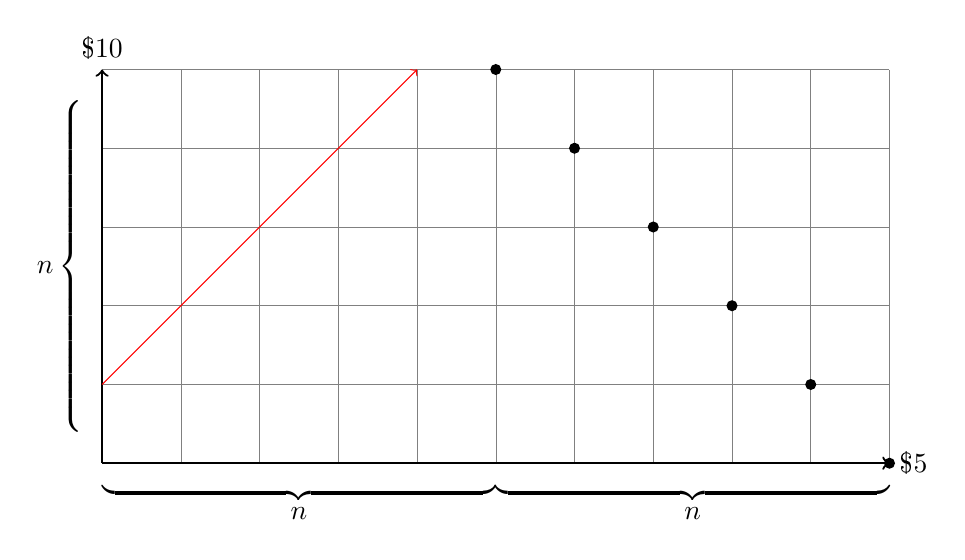
\begin{tikzpicture}
\draw[step=1cm,gray,very thin] (0,0) grid (10,5);
\draw[->,thick] (0,0) -- (10,0) node[right] {\$5};
\draw[->,thick] (0,0) -- (0,5) node[above] {\$10};
\node at (-0.34,2.5) {$\textstyle n \left\{\begin{array}{c}\\ \\ \\ \\ \\ \\ \\ \\ \\ \\\end{array}\right.$};
\draw[red, ->] (0,1) -- (4,5);
\fill[black] (5,5) circle (2pt);
\fill[black] (6,4) circle (2pt);
\fill[black] (7,3) circle (2pt);
\fill[black] (8,2) circle (2pt);
\fill[black] (9,1) circle (2pt);
\fill[black] (10,0) circle (2pt);
\node at (2.5,-0.5) {$\underbrace{\phantom{\rule{5cm}{0pt}}}_{\textstyle n}$};
\node at (7.5,-0.5) {$\underbrace{\phantom{\rule{5cm}{0pt}}}_{\textstyle n}$};
\end{tikzpicture}
\end{center}

\begin{center}
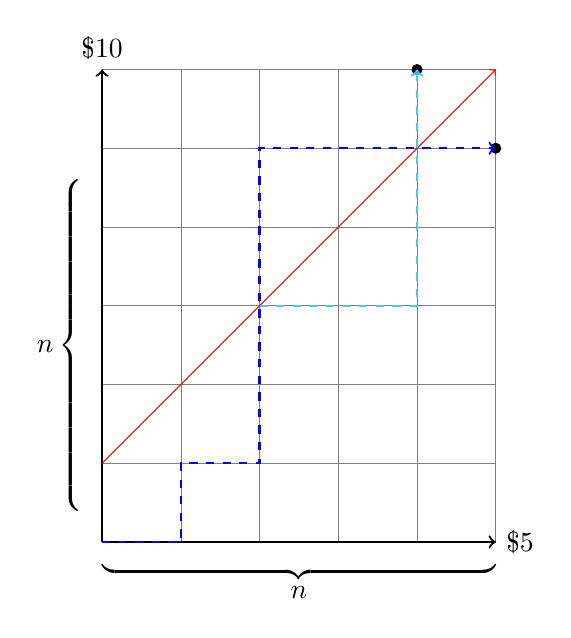
\begin{tikzpicture}
\draw[step=1cm,gray,very thin] (0,0) grid (5,6);
\draw[->,thick] (0,0) -- (5,0) node[right] {\$5};
\draw[->,thick] (0,0) -- (0,6) node[above] {\$10};
\node at (-0.34,2.5) {$\textstyle n \left\{\begin{array}{c}\\ \\ \\ \\ \\ \\ \\ \\ \\ \\\end{array}\right.$};
\draw[red, ->] (0,1) -- (5,6);
\fill[black] (5,5) circle (2pt);
\fill[black] (4,6) circle (2pt);
\draw[blue, dashed, thick, ->] (0,0) -- (1,0) -- (1,1) -- (2,1) -- (2,2) -- (2,3) -- (2,4) -- (2,5) -- (3,5) -- (4,5) -- (5,5);
\draw[cyan!70!white, dashed, thick, ->] (2,3) -- (3,3) -- (4,3) -- (4,5) -- (4,6);
\node at (2.5,-0.5) {$\underbrace{\phantom{\rule{5cm}{0pt}}}_{\textstyle n}$};
\end{tikzpicture}
\end{center}

\end{document}